\documentclass{article}
\usepackage[utf8]{inputenc}
\usepackage{amsmath}
\usepackage[spanish,es-tabla]{babel}
\usepackage{graphicx}
\usepackage{amssymb, amsmath, amsbsy} 
\usepackage{mathtools}
\usepackage{multicol}
\usepackage{scalerel,amsmath}
\usepackage [ spanish ]{babel}
\usepackage [utf 8]{inputenc }
\usepackage {graphicx }
\usepackage[a4paper]{geometry}
\title{TP1 -1}
\author{mendozachacon.t }
\date{May 2021}

\begin{document}

\maketitle

\section{Pregunta 1}


 
\begin{enumerate}
		
\item  \textbf{Equilibrio del mercado de trabajo:} Bajo la información en t-1, los agentes eligen $l_t$ óptimo del siguiente periodo (esto es equivalente para las firmas).
$$
	E_{t-1}[\frac {\gamma}{c_t}(1-\alpha)\frac {y_t}{e_t l_t}-\eta]=0
$$

\item \textbf{Decisión intratemporal}:  Si  la economía no cambia entre lo que es antes conocidos los estados de la naturaleza de la tecnología y la inversión, los agentes elegirán trabajar exactamente lo planeado en el periodo t-1. De lo contrario, estos ajustarán su decisión óptima mediante el esfuerzo.
$$
	\frac{\gamma}{c_t}(1-\alpha)\frac{y_t}{e_t l_t}-\eta=\frac{\theta(e_t-1)}{l_t}
 $$

\item \textbf{Euler de consumo:} El beneficio marginal esperado de consumir una unidad hoy(dado el shock en la inversión) debe igualar el beneficio marginal de consumir una unidad mañana.
$$
\frac{1}{c_t\xi_t}=\beta[\alpha\frac{\gamma}{c_{t+1}}\frac{y_{t+1}}{k_{t+1}}+(1-\delta) \frac{\gamma}{c_{t+1}} \frac{1}{xi_{t+1}}
$$


\item \textbf{Restricción:} El producto debe ser igual al consumo más la inversión.
$$
	y_t=c_t+i_t
	$$

\item \textbf{Ley de movimiento del capital:}El capital del siguiente periodo se descompone en: capital depreciado del periodo pasado más inversión (esta última sujeto a un shock con proceso estocástico)
$$
	k_{t+1}=(1-\delta)k_t+\xi_ti_t
$$
\item \textbf{Producto}: Función de producción cobb-douglas sujeto a un shock tecnológico (estocástico) . La participación del capital es $\alpha$ y la del trabajo por esfuerzo (1-$\alpha$).
$$
y_t=A_t k_t^\alpha (e_tl_t)^{1-\alpha}
$$
\item Proceso estocástico del shock tecnológico
$$
\ln A_t=\rho \ln A_{t-1}+u_1
$$
\item Proceso estocástico del shock en la inversión
	$$
	\ln \xi_t=\rho_\xi \ln \xi_{t-1}+u_2
	$$
\end{enumerate}

Interpretación de gráficos ante un shock en la tecnología:
 
\begin{itemize}

\item \textbf{Imagen 1 y 2 (A e Y) :} Tanto el producto como la fuente del shock (A) aumentan de manera proporcional al valor de este mismo, dada la función de producción. A medida que pasan más periodos, el shock converge a su media 0 y el producto y la tecnología vuelven a su estado estacionario.
\begin{figure}[h]
	\centering
	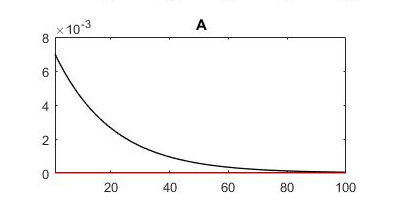
\includegraphics[width=0.5\linewidth]{a_1}
	\caption{shock tecnológico}
	\label{fig:a1}
\end{figure}

\begin{figure}[h]
	\centering
	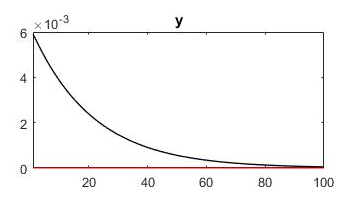
\includegraphics[width=0.4\linewidth]{y_2}
	\caption{}
	\label{fig:a1}
\end{figure}
\newpage
\item \textbf{Imagen 3 y 4 (C y K):} Durante los primeros periodos posteriores al shock, tanto el consumo como el capital aumentan. Esto se debe a que mayor producto hace posible mayores niveles de consumo y hacen los factores más productivos. Posterior a esto, ambos bajan fuertemente conforme el shock vuelve a su estado natural, llegando a su estado estacionario en el largo plazo

\begin{figure}[h]
	\centering
	\includegraphics[width=0.5\linewidth]{"MicrosoftTeams-image (6)"}
	\label{fig:microsoftteams-image-6}
\end{figure}
\begin{figure}[h]
	\centering
	\includegraphics[width=0.5\linewidth]{"MicrosoftTeams-image (8)"}
	\caption{}
	\label{fig:microsoftteams-image-8}
\end{figure}


\item \textbf{Imagen 4 (I)}: La inversión, por su parte, aumenta en el periodo del shock por la misma razón que el capital (aumento en la productividad de los factores). Sin embargo, cae fuertemente conforme avanza el tiempo,  dado que cada vez el shock se acerca a su estado natural y a su vez hay cada vez más capital acumulado. Por esta misma razón, incluso hay un punto en que la inversión baja de su estado estacionario, con el propósito de converger al capital de estado estacionario.
\begin{figure}[h!]
	\centering
	\includegraphics[width=0.5\linewidth]{"MicrosoftTeams-image (7)"}
	\caption{}
	\label{fig:microsoftteams-image-7}
\end{figure}

\item \textbf{(L y E)}: El esfuerzo experimenta un alza en el periodo inmediato del shock, dado que la productividad marginal aumenta. Sin embargo, vuelve rápidamente a su estado estacionario. Finalmente, el trabajo también sube pero sufre una caída más suave que el esfuerzo, incluso llegando por debajo de su estadio estacionario, para volver paulatinamente a su estado estacionario en el largo plazo.
    
 \begin{figure}[h!]
 	\centering
 	\includegraphics[width=0.9\linewidth]{"MicrosoftTeams-image (10)"}
 	\caption{}
 	\label{fig:microsoftteams-image-10}
 \end{figure}
 
\end{itemize}
Shock en la inversión:
\begin{figure}[h!]
	\centering
	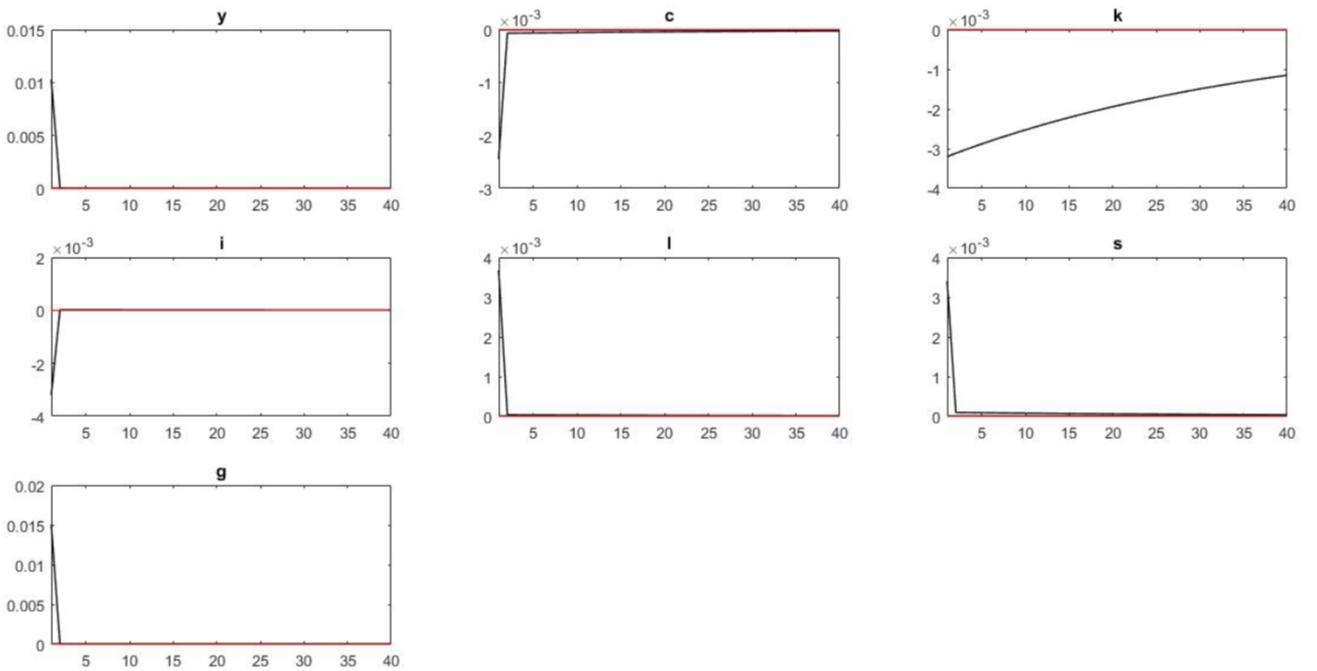
\includegraphics[width=1.2\linewidth]{shockinv}
	\label{fig:w3}
\end{figure}
\begin{itemize}
\item  
\end{itemize}

\section{Pregunta 2}

\subsection{Condiciones de equilibrio}
\begin{enumerate}
	\item 
	$$
	\eta=(1-\alpha)\frac{1}{c_t} \frac{y_{t}} {l_{t}}
	$$ 
	\item El precio relativo del capital debe igualar el costo marginal de la inversión en t.
	$$
	\frac{\mu_{t}}{\lambda_{t}}=-(1+2 \phi i_{t})
	$$
	\item Condición de óptimo de la intensidad de uso del capital: En el óptimo, un cambio marginal en el producto respecto a la tasa del uso de capital, debe igualar una fracción del capital utilizado en el periodo t.  
	$$
	\alpha\frac{y_t}{s_t}-\nu s_tk_t=0
	$$
	\item Euler de consumo: El costo marginal de ahorrar una unidad hoy debe ser equivalente al beneficio marginal generado en el siguiente periodo (descontado). 
	$$
	\frac{2\phi i_t+1}{c_t} = \beta \frac{1}{c_{t+1}}\left[ \frac{\alpha y_{t+1}}{k_{t+1}}-0.5v(s^2_{t+1}-1) + (1-\delta)(2\phi i_{t+1} +1)\right]
	$$
	
	
	\item Un shock positivo en el gasto publico afectara negativamente el consumo y la inversión, lo que a su vez tendrá repercusiones en la intensidad de uso del capital. 
	
	
	$$
	g_t=\phi \epsilon_t
	$$
	\item 
	$$
	\ln A_{t}=\theta_{A} \ln A_{t-1}+\epsilon_{A t}
	$$
	\item 
	$$
	y_{t}=A_{t} l_{t}^{1-\alpha}\left(k_{t} s_{t}\right)^{\alpha}
	$$
	\item 
	$$ 
	y= c_t+i_t(1+\phi i_t) + 0.5v(s^2_t-1)k_t + g_t
	$$
	\item
	$$
	k_{t+1}=i_{t}+(1-\delta) k_{t}
	$$
\end{enumerate}
\subsection{Steady State}
\begin{equation}
	\frac{1}{c}(1 - \alpha)\frac{y}{l} = \eta
\end{equation}
\begin{equation}
	p_k = -(2\phi i+1)
\end{equation}
\begin{equation}
	\alpha y - \nu k = 0
\end{equation}
\begin{equation}
	(2\phi i+1) = \beta \left[ \alpha \frac{y}{k} + (1-\delta)(2\phi i+1) \right]
\end{equation}
\begin{equation}
	g = 0
\end{equation}
\begin{equation}
	A = 1
\end{equation}
\begin{equation}
	y = k^\alpha l^{1-\alpha} = c + i(1+\phi i)
\end{equation}
\begin{equation}
	i = \delta k
\end{equation}
\newpage
\begin{figure}[h]
	\centering
	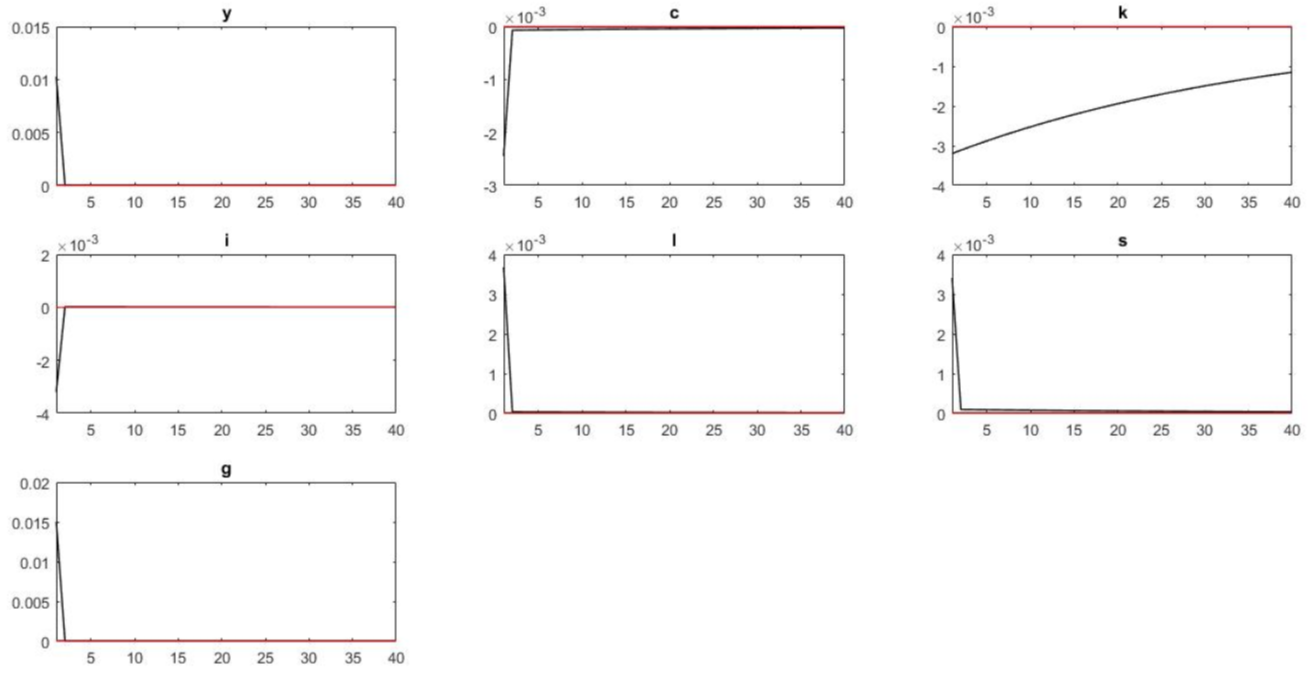
\includegraphics[width=1.2\linewidth]{shockgasto}
	\label{fig:a}
\end{figure}
\begin{figure}[h]
	\centering
	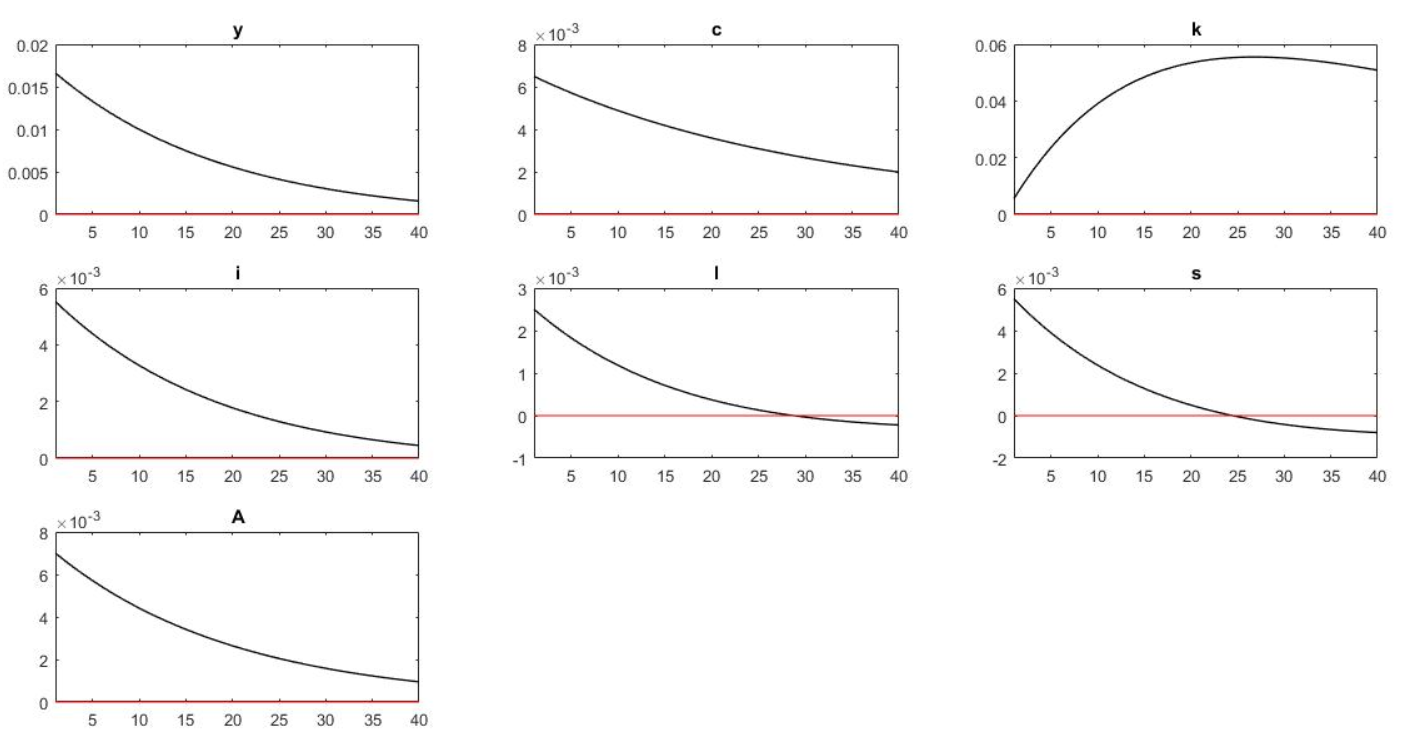
\includegraphics[width=1.2\linewidth]{schocktec2}
	\label{fig:a}
\end{figure}

\newpage
\section{Pregunta 3}
\subsection{Lagrangiano-CPO}
\subsection{Condiciones de equilibrio}
\begin{equation}
	 {\dfrac{z_t}{C_t}}(1-\alpha){\dfrac{Y_t}{N_t}}=\eta \nonumber
\end{equation}

\begin{equation}
	\dfrac{z_t}{C_t}[1-\alpha{\dfrac{Y_t}{K_t}}{\dfrac{1}{\nu\delta s_t^\nu}}(1-\dfrac{\kappa}{2}({\dfrac{I_t}{I_{t-1}}-1})^2)-\kappa(\dfrac{I_t}{I_{t-1}}-1)(\dfrac{I_t}{I_{t-1}})]=\beta{\dfrac{z_{t+1}}{C_{t+1}}}\alpha{\dfrac{Y_{t+1}}{K_{t+1}}}{\dfrac{1}{\nu\delta s_{t+1}^\nu}}\kappa({\dfrac{I_{t+1}}{I_{t}}})^2({\dfrac{I_{t+1}}{I_{t}}}-1) \nonumber
\end{equation}

\begin{equation}
	{\dfrac{z_t}{C_t}}=\beta[{\dfrac{z_{t+1}}{Q_{t+1}}}+{\dfrac{z_{t+1}}{C_{t+1}}}] \nonumber
\end{equation}






\begin{equation}
	\omega_{t}\left(s_{t} K_{t}\right)^{\alpha} N_{t}^{1-\alpha}=y_t \nonumber
\end{equation}

\begin{equation}
	C_t+I_t+Q_{t+1}-Q_t=Y_t \nonumber
\end{equation}

\begin{equation}
	K_{t+1}=I_t[1-\dfrac{\kappa}{2}({\dfrac{I_t}{I_{t-1}}-1})^2]+(1-\delta s_t^\nu)K_t \nonumber
\end{equation}


\newpage
\begin{figure}[h!]
	\centering
	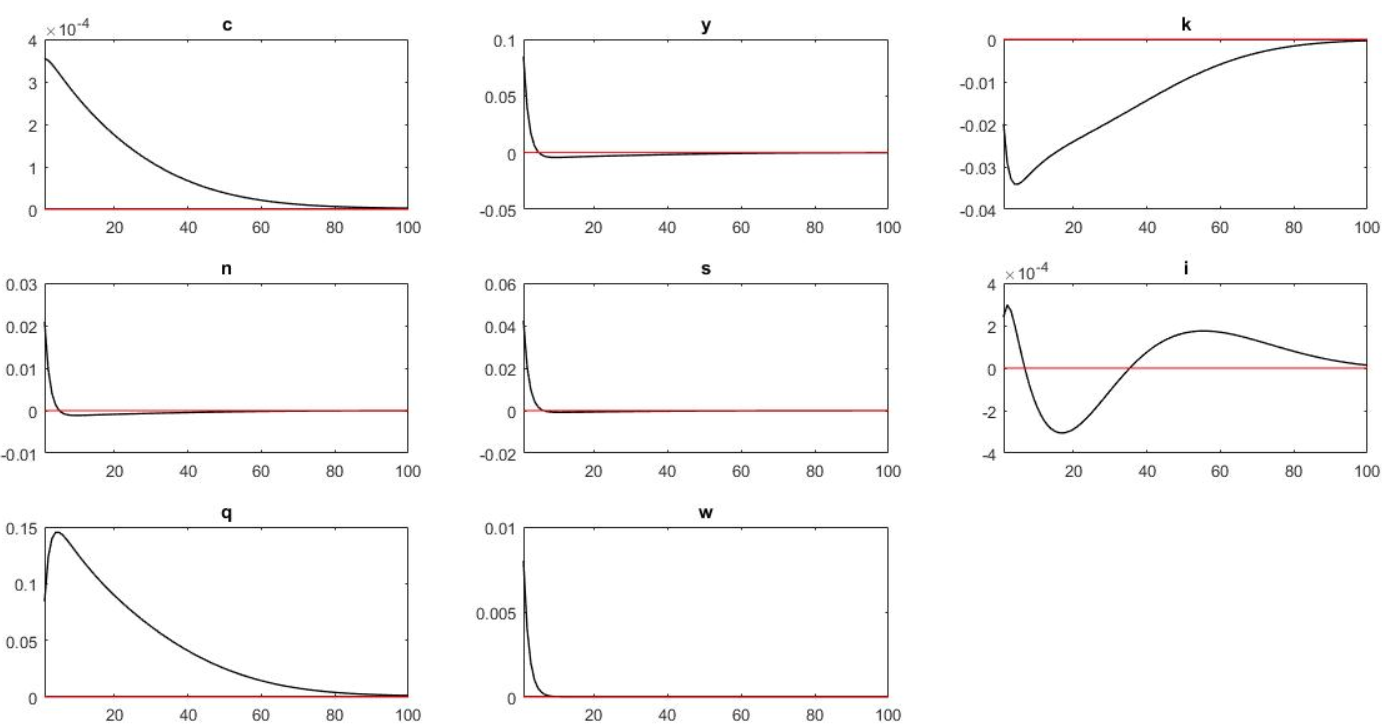
\includegraphics[width=1.2\linewidth]{shockprefer}
	\label{fig:w3}
\end{figure}



\newpage
\begin{enumerate}
\item shock tecnológico	
	\end{enumerate}

\begin{figure}[h!]
	\centering
	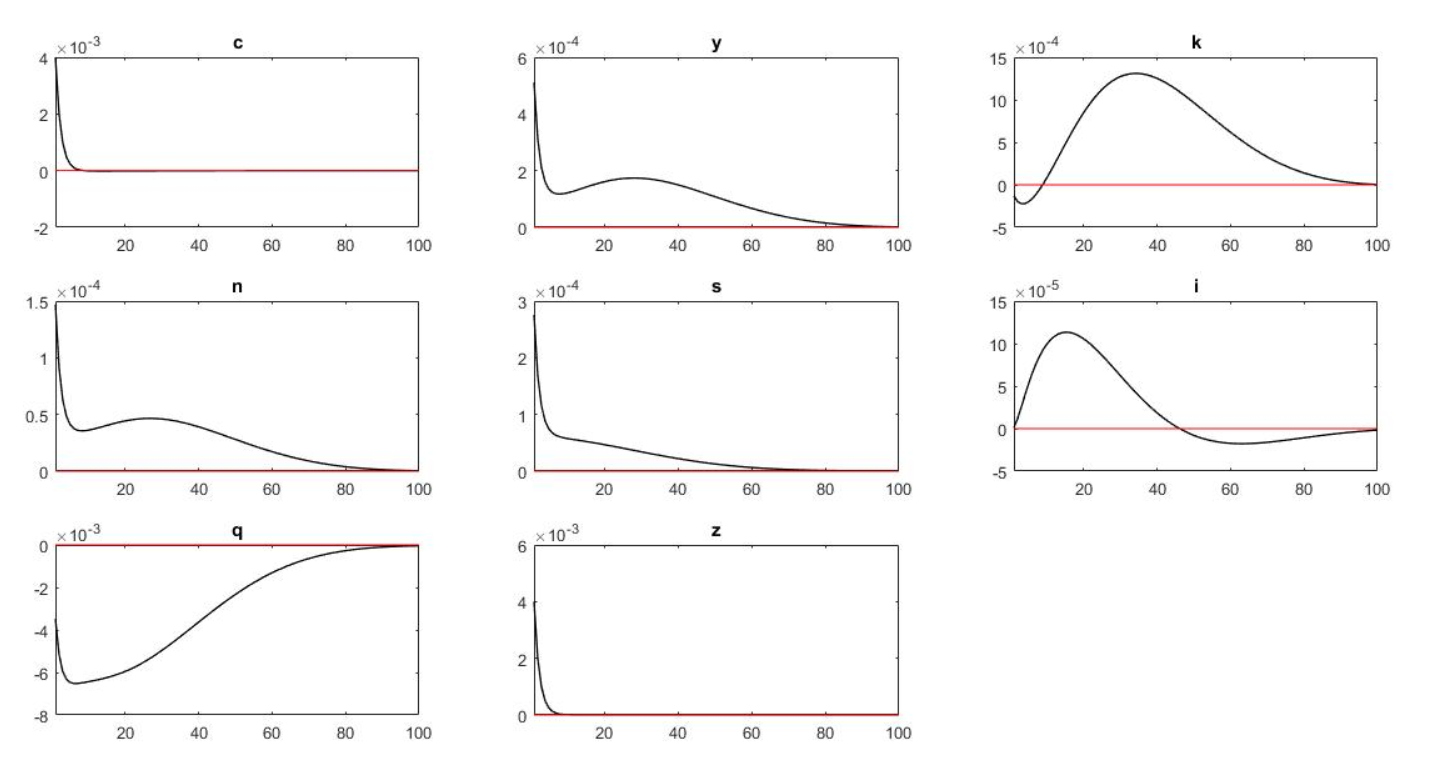
\includegraphics[width=1.2\linewidth]{shocktec}
	\label{fig:w3}
\end{figure}


\end{document}
